\section{粗視化分子動力学法(CGMD法)の概要}
%--------------------
\begin{figure}[h]
	\begin{center}
	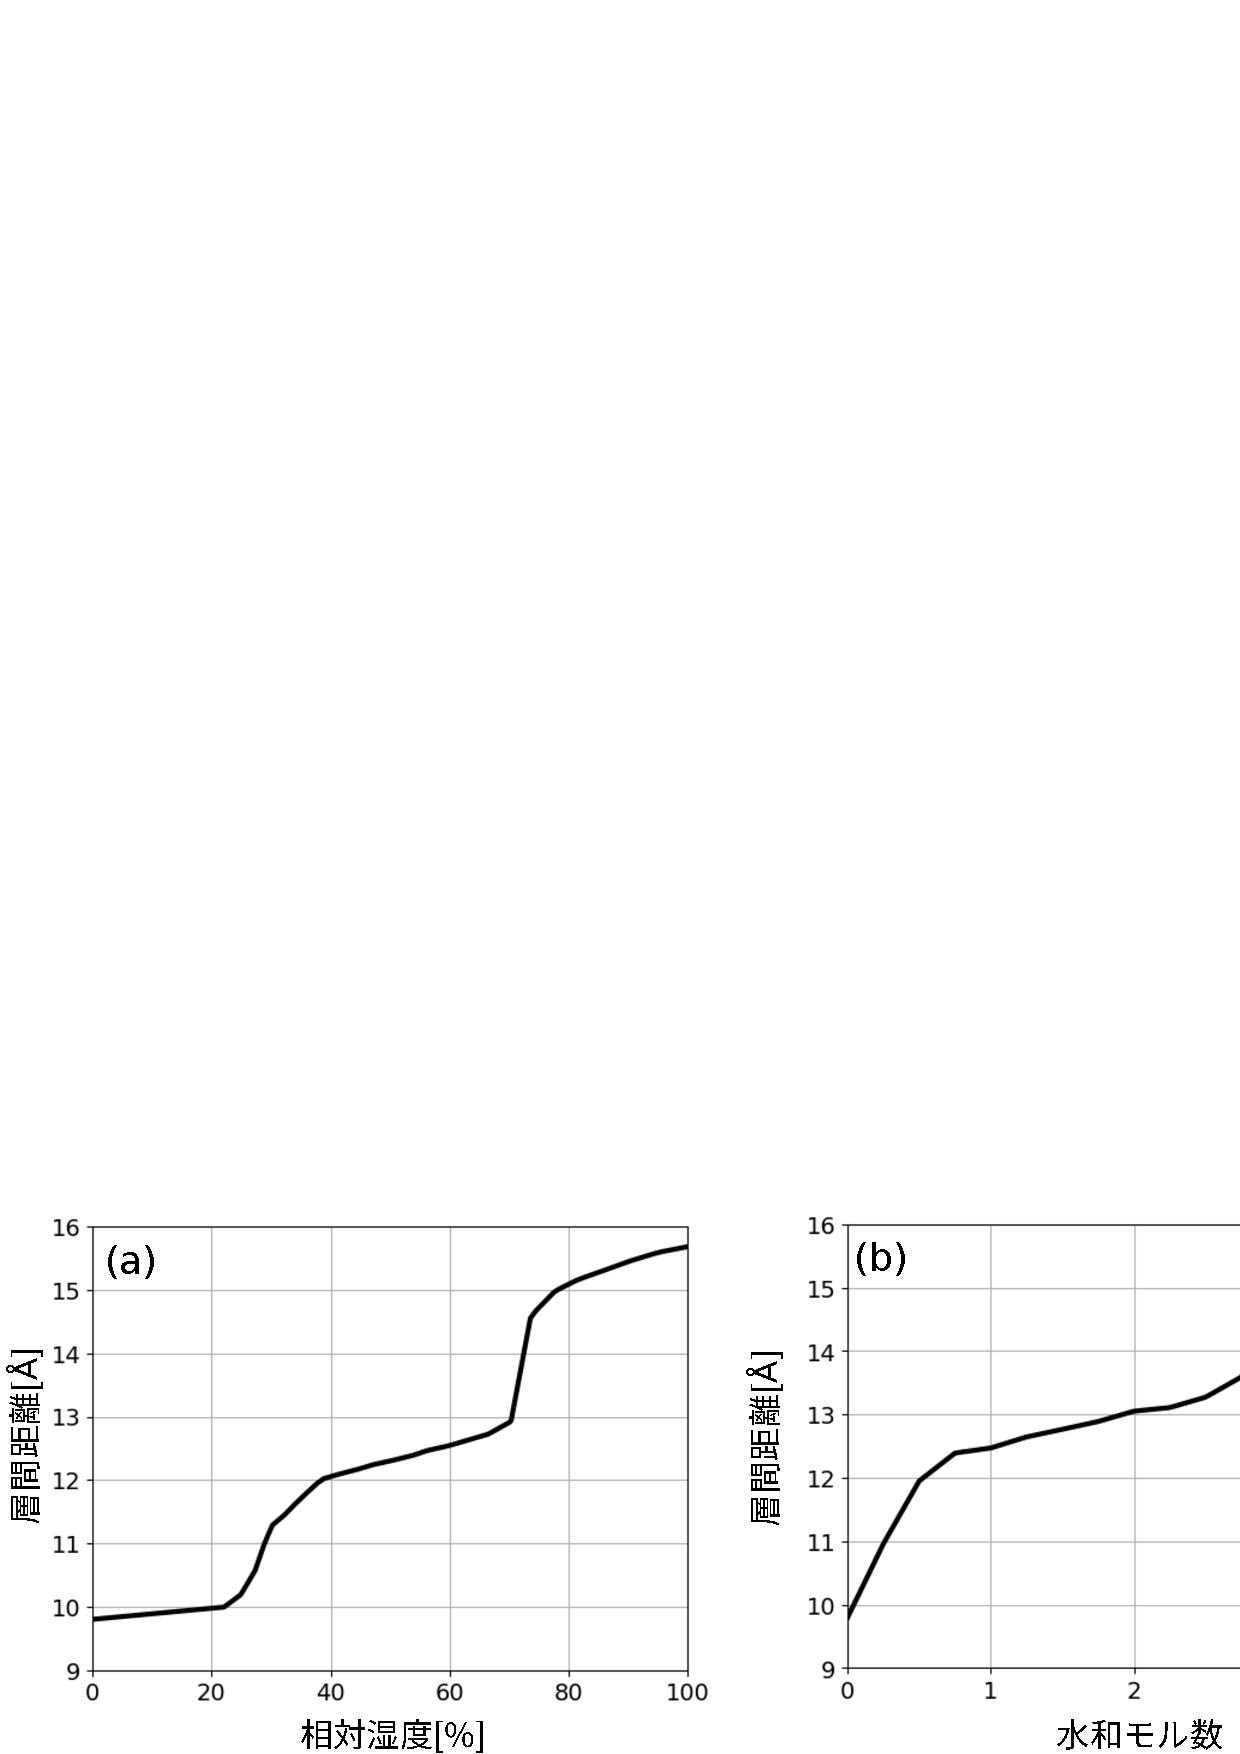
\includegraphics[width=1.0\linewidth]{Figs/fig1.pdf} 
	\end{center}
	\caption{
		Na型モンモリロナイトの膨潤挙動.
		(a) X線回折試験で得られた相対湿度と層間距離の関係(諸留,河村2009\cite{Morodome}
		から再現).(b) 全原子MD計算で得れられた水和モル数と層間距離の関係
		(森本ら2023\cite{Morimoto}). 
	} 
	\label{fig:fig1}
\end{figure}
%--------------------
\begin{figure}[h]
	\begin{center}
	\includegraphics[width=1.0\linewidth]{Figs/fig2.pdf} 
	\end{center}
	\caption{
		Na型モンモリロナイトの膨潤データから作成した
		水和エネルギーモデルと水和モル数の関係.
		(a)化学ポテンシャル$\mu(n)$, (b)水和エネルギーの非線形成分$\delta G_{hyd}(n)$.
	} 
	\label{fig:fig2}
\end{figure}
%--------------------
%--------------------
\subsection{粒子間相互作用力}
CGMD法では,粗視化粒子に作用する力として分子内力と分子間力の2つを与える.
分子内力は,粗視化粒子を結合して一つの分子として振る舞うように剛性を与える
もので,本CGMD法では同一分子内で隣接する粗視化粒子を線形バネで結合すること
によって与えている.そのため,無応力状態では一つの分子を表現する粗視化粒子群
は直線上に整列する.
分子間力はファンデルワールス力の基本的なモデルであるレナード-ジョーンズ対ポテンシャル
(以下LJポテンシャル呼ぶ):
\begin{equation}
	U(\fat{x}_i,\fat{x}_j; \sigma) 
	= 4 \varepsilon 
	\left\{ 
	\left(\frac{\sigma}{r_{ij}}\right)^{12}
	-
	\left(\frac{\sigma}{r_{ij}}\right)^6
	\right\}, \ \ \left( r_{ij}=\left| \fat{x}_i-\fat{x}_j\right| \right)
	\label{eqn:LJ}
\end{equation}
で与える.
ここで,$\fat{x}_i$と$\fat{x}_j$は,それぞれ第$i$および第$j$番目の粗視化粒子の位置を,
$\varepsilon$と$\sigma$は,LJポテンシャルのパラメータを表す.$\varepsilon$は
\begin{equation}
	\varepsilon=1.0\times 10^{-19}, \ \ [{\rm Nm}]
	\label{eqn:eps_of_LJ}
\end{equation}
であり,$\sigma$は以下に述べるように粗視化粒子に水和した水分量を表す変数として用いる.

LJポテンシャルは粒子間距離$r_{ij}$が小さいときに斥力を,大きいときに引力を粒子間に作用させる.
引力と斥力は概ね$r_{ij}=1.1\sigma$を境に切り替わる.
斥力が作用する領域では$r_{ij}\rightarrow 0$に向けて斥力が急増する.
従って,$r_{ij}=\sigma$は粗視化粒子の接近限界とみなすことができる.
水を非圧縮性物質とみなせば,粗視化粒子の接近限界は粘土分子が当該位置でもつ
水和水量で決まる.いま,粒子$i$のもつ水和層の厚みが$s_i$,
粒子$j$のそれが$s_j$であったとする.無水状態での粘土分子層の厚さを$\sigma_0$とすれば,
粗視化粒子の接近限界$\sigma$は次の式で与えられる.
\begin{equation}
	\sigma=\sigma_0 +s_i+s_j
	\label{eqn:}
\end{equation}
このことより,粗視化粒子の有する水和水層の厚さ$s_i$を定めればLJポテンシャルの
特性距離$\sigma$が決まり,水和水の量や分布に応じた粒子間相互作用を与えることができる.
CGMD法では,各粗視化粒子は位置$\fat{x}$と速度$\fat{v}$,向き$\fat{n}$を属性として持つ.
ここで,粘土分子の一方の面を正方向$\fat{n}$とし,その反対の方向を$-\fat{n}$とすれば,
これら2つの方向それぞれに水和水が存在するため,$\pm\fat{n}$方向の水和水層厚を
区別する場合$s^\pm$, 文脈から明らかな場合は$\pm$を省略して$s_i$などと書く.
ここに,$i$は粗視化粒子番号を意味する.粒子番号についても明示する必要の無い場合は省略し
単に$s$と書く.これら$\fat{x},\fat{v},\fat{n}$および$s$は全て未知量である.
これらのうち$\fat{x}$と$\fat{v}$は,運動方程式:
\begin{equation}
	m\dot{ \fat{v}}=\fat{F}_K+\fat{F}_{LJ}, \ \ \fat{v}=\dot{\fat{x}}
	\label{eqn:eq_motion}
\end{equation}
を時間積分することで与えられた初期状態から繰り返し状態を更新する.
なお,$m$は粗視化粒子の質量を, $\fat{F}_K$と$\fat{F}_{LJ}$は,
それぞれ分子内および分子間力を表す.粒子の向き$\fat{n}$は,分子を構成する
粗視化粒子の位置座標から各粒子位置での接ベクトルを求め,それに直交する方向として定める.
水和水層の厚さ$s$は,後に述べるように水和エネルギーと粒子間相互作用エネルギー
の停留条件から決定する.水和水層の厚さ$s$とX線回折試験から求められている
膨潤状態および層間距離は表\ref{tbl:tbl_sig}の通りである.
\begin{table}[h]
	\begin{center}
	\caption{分子間相互作用ポテンシャルにおける特性距離と膨潤状態の対応.}
	\vspace{3mm}
	\begin{tabular}{c||c|c|c|c|c}
		膨潤状態 & 0層 & 1層 & 2層 & 3層 & $\cdots$\\
		\hline
		特性距離(層間距離)$\sigma$[{\rm nm}]& 0.9 & 1.2 & 1.5 & 1.8 & $\cdots$ \\
		\hline
		水和水層厚$s$[{\rm nm}] & 0.0 & 0.15 & 0.30 & 0.45 & $\cdots$
	\end{tabular}
	\label{tbl:tbl_sig}
	\end{center}
\end{table}
%--------------------
\subsection{水分に関係したエネルギー}
粘土含水系を表現する粗視化粒子系は,水分の配置や量に応じて系全体がもつエネルギーを変化させる.
水分の量や配置に依存するエネルギーには,次のものが考えられる.
\begin{itemize}
\item
	粗視化粒子間相互作用のエネルギー(LJポテンシャル)$U_{LJ}$
\item
	水和エネルギー$U_{hyd}$
\item
	系内の水分量に依存するエネルギー$U_N$
\end{itemize}
粒子間相互作用エネルギー$U_{LJ}$は,LJポテンシャル(\ref{eqn:LJ})の特性距離$\sigma$を
通じて水分位置と量の影響を受ける.上記$U_{LJ}$は粒子径の全ポテンシャルエネルギーである
ため,CGMDを法では次の式で与えられる.
\begin{equation}
	U_{LJ}=\sum_{i \neq j} U(\fat{x}_i,\fat{x}_j; \sigma) 
	\label{eqn:}
\end{equation}
$U_{hyd}$は,水分が粘土分子の表面や層間に水和することによるエネルギー変化を表す.
水和水層の厚さが$s$における粗視化粒子の水和エネルギーを$u(s)$とすれば,
$U_{hyd}$は
\begin{equation}
	U_{hyd} =\sum_{\alpha=\pm} \sum_{i} u(s_i^{\alpha})
	\label{eqn:Uhyd_tot}
\end{equation}
と表される.なお,ここでは水和エネルギーの基準を無水状態にとり,$u(0)=0$としている.
モンモリロナイトは大きなは膨潤や膨潤圧を生じることからも明らかなように,
湿潤環境下で強い水和が生じる.従って,水和エネルギー$U_{hyd}$は$U_{LJ}$との比較において
無視できない.
最後に,$U_{N}$は系内に存在する水分量の変動だけに起因したエネルギーを表す.
一般に,系外から物質を持ち込み,系の組成を変化させるためにはエネルギーが必要とされ,
$U_N$は系内外での水分の授受に関するものである.
水分粘土含水系と環境をひとまとめにして見たとき,粘土含水系内の水分と環境中の水分では
濃度が異なる.そのため粘土含水系は,系内での水分位置によらず,系外との濃度差に
起因したエネルギー$U_N$を持つ.
CGMD法では水分を粗視化粒子の属性として表現するため,水分や水分子間の相互作用力や
相互作用エネルギーは計算されない.従って,これら$U_{hyd}$や$U_{N}$はモデルや
計算条件として別途与える必要がある.

熱力学の第二法則に従えば,水分量と位置の自発的変化はこれら3つのエネルギーの和
\begin{equation}
	E=U_{LJ}+U_{hyd}+U_{N}
	\label{eqn:}
\end{equation}
が減少する方向に起きる.このことは,水分位置と量の変化に関する全微分を使って
\begin{equation}
	dE = dU_{LJ}+dU_{hyd}+dU_N <0
	\label{eqn:dE}
\end{equation}
と表され,平衡状態では停留条件$dE=0$満足する.なお,$U_N$は水分配置に依らないため,
系内の水分子数を$N$とすれば,
\begin{equation}
	dU_N=\mu dN, \ \ \left(  \mu:=\frac{\partial U_N}{\partial N}\right)
	\label{eqn:}
\end{equation}
とできる.ここで$\mu=\frac{\partial U_N}{\partial N}$は水分に関する化学ポテンシャルを表す.
化学ポテンシャル一定のもとで計算を行う場合,式(\ref{eqn:dE})右辺の各項を計算し,
$dE<0$となる方向に水分状態を推移させる.この作業を繰り返し,最終的に停留条件$dE=0$
が満足される状態まで粗視化粒子径を緩和させれば,平衡状態における水分量と配置が決定できる.
その際,指定された化学ポテンシャルが$\mu>0$であれば,系内の水分が増加するとき$dN>0$で$U_N$も増加する.
これに対し水和エネルギー$U_{hyd}$は,水分量に関する負の減少関数のため,$dN>0$のとき$dU_{hyd}<0$である.
一方,$dU_{LJ}$は水分量の増加に対して正にも負にも成り得る.例えば,周囲の粒子から斥力を受ける
粗視化粒子に水分が追加されると,斥力はさらに大きくなりポテンシャル値も増加する.
逆に,粗視化粒子が疎に配置された状態で水分が追加されれば,粒子間の引力が増しポテンシャルは減少する.
このように,水和エネルギー$U_{hyd}$と水分量に関する$U_N$は相反する応答を示し,
ポテンシャルエネルギー$U_{LJ}$は状況に応じて増減方向が決まる.
平衡状態における水分量と配置は,これらのエネルギー変化が互いに拮抗する状態として決定される.
化学ポテンシャル$\mu$は定義上,その値が大きい場合,環境から水分を系内に取り込む際に要するエネルギーが大きい.
逆に$\mu$が小さく設定されていれば,わずかなエネルギーを供給するだけで系内に水分を取り込むことができる.
これを物理的な状況にあてはめると,前者は粘土含水系が置かれた環境の湿度が低い場合に,
後者は湿度が高い場合に相当する.環境の湿度が低い場合,そこから所定の水分を粘土含水系に
移すために要するエネルギーは湿度が高い場合よりも大きいことは明らかであろう.
以上のことから,化学ポテンシャルの逆数$\mu^{-1}$は 粘土含水系が置かれた環境の湿度の
高低に相当する指標とみなすことができる.

CGMD法では水分量を表す変数は,水和水層の厚さ$s$であり水分子数$N$ではない.そこで,
CGMD法への実装において,水分量に関するエネルギー$U_N$の変化を
\begin{equation}
	dU_N=\tilde \mu ds, \ \ \left( \tilde \mu =\mu \frac{dN}{ds} \right)
	\label{eqn:}
\end{equation}
と表し,$\tilde \mu$を与えて計算を行う.$\tilde \mu$と$\mu$は定数倍だけの差であるため,
以下では$\tilde \mu$も化学ポテンシャルと呼ぶことにする.ただし,$\mu$がエネルギーの次元を持つのに対し,
$\tilde \mu$はエネルギー/長さの次元を持つことに注意する.
\subsection{水和エネルギー}
平衡状態においてどの程度の水分が系内に取り込まれるかは,化学ポテンシャル$\mu$の大小だけでなく,
$U_{LJ}$や$U_{hyd}$との兼ね合いで決まる.特に,水分量に関するエネルギー$U_N$と増減が反転する
水和エネルギー$U_{hyd}$の影響は大きい.また,水和エネルギーは,粘土鉱物や層間イオン種による
吸水や膨潤挙動の違いを生むという意味でも重要である.
従って,水和エネルギーと膨潤挙動の関係を理解することが,適切な組織構造モデルを得る
ために必要と言える.
%
\subsubsection{単調モデル}
図\ref{fig:fig1}(a)に,昨年度の研究で用いた水和エネルギーモデルを示す.ここでいう
水和エネルギーモデルとは,粗視化粒子の各方向に水和した,水和水の層厚と水和エネルギーの
関係を指す.図\ref{fig:fig1}(a)の水和エネルギーモデルは次の式で与えられる.
\begin{equation}
	u(s)=-u_{\infty} \left(1-e^{-\gamma s} \right)
	\label{eqn:u_s}
\end{equation}
ここに,$s$は水和水層の厚さを,$s_b$は
\begin{equation}
	\frac{\left| u(s_b) \right|}{u_{\infty}}=\frac{1}{2}
	\label{eqn:u_sb}
\end{equation}
となる基準距離を,$u_{\infty}$は$s\rightarrow \infty$(無限膨潤)
での水和エネルギーの大きさを表す.
全水和エネルギー$U_{hyd}$を与える式(\ref{eqn:Uhyd_tot})の右辺は,
式(\ref{eqn:u_s})をはじめとする水和エネルギーモデルによって計算する.
式(\ref{eqn:u_sb})より
\begin{equation}
	e^{-\gamma s_b}=\frac{1}{2} \ \ \Rightarrow \ \
	\gamma=\frac{\log 2}{s_b}
	\label{eqn:}
\end{equation}
である.よって,$s_b$を与えれば$\gamma$が決まる.
図\ref{fig:fig1}(b)は,$u(s)$の勾配$u'(s)$を示したもので,
\begin{equation}
	u'(s)=\frac{du}{ds}=-\gamma u_{\infty} e^{-\gamma s}
	\label{eqn:ud_s}
\end{equation}
より,
\begin{equation}
	\frac{u'(s_b)}{u'(0)}=\frac{1}{2}
	\label{eqn:ud_half}
\end{equation}
で,$s=s_b$において水和エネルギー関数の勾配も半減することが分かる.
このような水和エネルギーモデルを用いる理由は以下の通りである.
\begin{itemize}
\item
	単調減少する関数であること
\item
	$u(0)=0$かつ$s\rightarrow \infty$で有界であること
\item
	勾配の大きさが単調減少し,$s\rightarrow \infty$で0に収束すること
\end{itemize}
モンモリロナイトは水分子を強く水和し,最終的には分散状態に至る.
このことから,水和エネルギーは大局的に減少する関数でなければならない.
ただし,水和エネルギーが無限大となることは物理的でないため,2番目の条件を課す.
3番目の条件は,水和量が少ない程,より強く水分を吸着することを意味する.
式(\ref{eqn:u_s})は,これらの条件を満たすもののうち,単純かつ少数のパラメータで
規定できるものとして,昨年度採用したものである.以下ではこれを,単調モデルと呼ぶ.
なお,今回の計算では,基準距離を$s_b=0.1$nmとしている.
%
\subsubsection{振動モデル}
X線回折試験の結果から,Na型モンモリロナイトは相対湿度の増加に対して階段状に
層間距離を変化させることが知られている.層間距離は,概ね水分子整数個分程度となり,
水分子$n$個相当の層間距離にある状態を$n$層膨潤と呼ぶ.
Na型モンモリロナイトは0層膨潤から1層,2層膨潤と推移し,例えば1.5層といった
中間的な膨潤状態を取ることは少ない.このような挙動は水和エネルギー関数に
単調モデルを用いた場合に生じ得ない.これは,整数次の膨潤状態に相当する
水和水層厚で,水和エネルギー関数が何ら特別な特徴を持たないためである.
そこで,水分子サイズに相当する周期で変化する振動成分を単調モデルに加えた
水和エネルギーモデルを用いることで,どのように膨潤挙動の違いが現れるかを調べる.

$n$層($n=1,2,\dots$)膨潤状態における水和水層の厚さ$s$は,
表\ref{tbl:tbl_sig}に示すように,0.15nmの倍数である.
そこで,周期0.15nmの振動成分を単調モデルに加えることを考える.
図\ref{fig:fig2}(a)に,黒の実線でこの方法で作成した振動成分を有する
水和エネルギーモデルを示す.以下,この水和エネルギーモデルを振動モデルと呼ぶ.
単調モデルに加えたで振動成分は,同図(b)に緑の実線で示したものである.
これは,周期$H=$0.15nmの三角波を平滑化したもので,元になる三角波は
周期毎に一定割合で減衰させている.
ここで,単調モデルを$u_0(s)$,これに加えた平滑化した減衰三角波成分を$\Delta u(s)$
とすれば,振動モデルは
\begin{equation}
	u(s)=u_0(s)+ \Delta u(s)
	\label{eqn:}
\end{equation}
と表される.単調モデルは,大きさを表す項$u_{\infty}$と,関数系を決める無次元の項
$\bar u_0$の積で,
\begin{equation}
	u_0(s)=u_{\infty} \bar{u}(s), \ \ (\bar{u}(s)=-(1-e^{-\gamma s}))
	\label{eqn:}
\end{equation}
と書くことができる.振動成分$\Delta u(s)$の詳細は,以下のようである.


はじめに,周期関数の基本区間を$[0,H)$とし,この区間における高さ1の単一の三角波を
\begin{equation}
	V_0(s)=\left\{
		\begin{array}{cc}
			s/H & (0\leq s < H) \\
			0 & ({\rm otherwise})
		\end{array}
	\right.
	\label{eqn:V0}
\end{equation}
と書く.これを平行移動して順次加えることで,$s\geq 0$における周期関数$V(s)$が次の
ように得られる.
\begin{equation}
	V(s)=\sum_{k=0}^{\infty} \beta ^{k} V_0(s-kH)
	\label{eqn:Vs}
\end{equation}
ここで,$\beta(<1)$は減衰率で,隣接する三角波の振幅比を与えるパラメータである.
$V(s)$は$s=kT$において不連続であるため,ガウス分布等を重み関数w(s)として移動平均
\begin{equation}
	\tilde V(s)=\int V(t)w(s-t)dt
	\label{eqn:mv_ave}
\end{equation}
で平滑化し,連続かつ滑らかな関数$\tilde V(s)$にする.
$V_0(s)$の平滑化を$\tilde V_0(s)$とすれば,平滑化された減衰三角波は
\begin{equation}
	\tilde V(s)=\sum_{k=0}^{\infty} \beta ^{k} \tilde V_0(s-kH)
	\label{eqn:Vst}
\end{equation}
と書ける.式(\ref{eqn:Vst})は無次元の関数なので,これを単調成分$u_0(s)$の
無次元項$\bar{u}(s)$と比率$\alpha$で加えるために,
$\Delta u(s)=u_\infty\alpha \tilde V(s)$とする.
以上より,振動モデルを与える式は次のように表される.
\begin{equation}
	u(s)=u_0(s)+ \alpha \tilde V(s)= u_{\infty}\left\{ 
	\bar{u}(s)+ \alpha \sum_{k=0}^{\infty} \beta ^{k} \tilde V_0(s-kH)
	\right\}
	\label{eqn:us_triwv}
\end{equation}
式(\ref{eqn:us_triwv})は3つのパラメータ$u_{\infty},\alpha$および$\beta$で
定義される.$u_{\infty}$は$s\rightarrow \infty$での水和エネルギーの大きさを,$\alpha$は
単調成分と振動成分の比を,$\beta$は振動成分の減衰率をそれぞれ表す.
次節の計算例では,これらのパラメータは次のように与える.
\begin{equation}
	\alpha=0.22, \ \ \beta=0.6, \ \ H=0.15 \ \ [{\rm nm}]
	\label{eqn:}
\end{equation}
%--------------------
\begin{figure}[h]
	\begin{center}
%	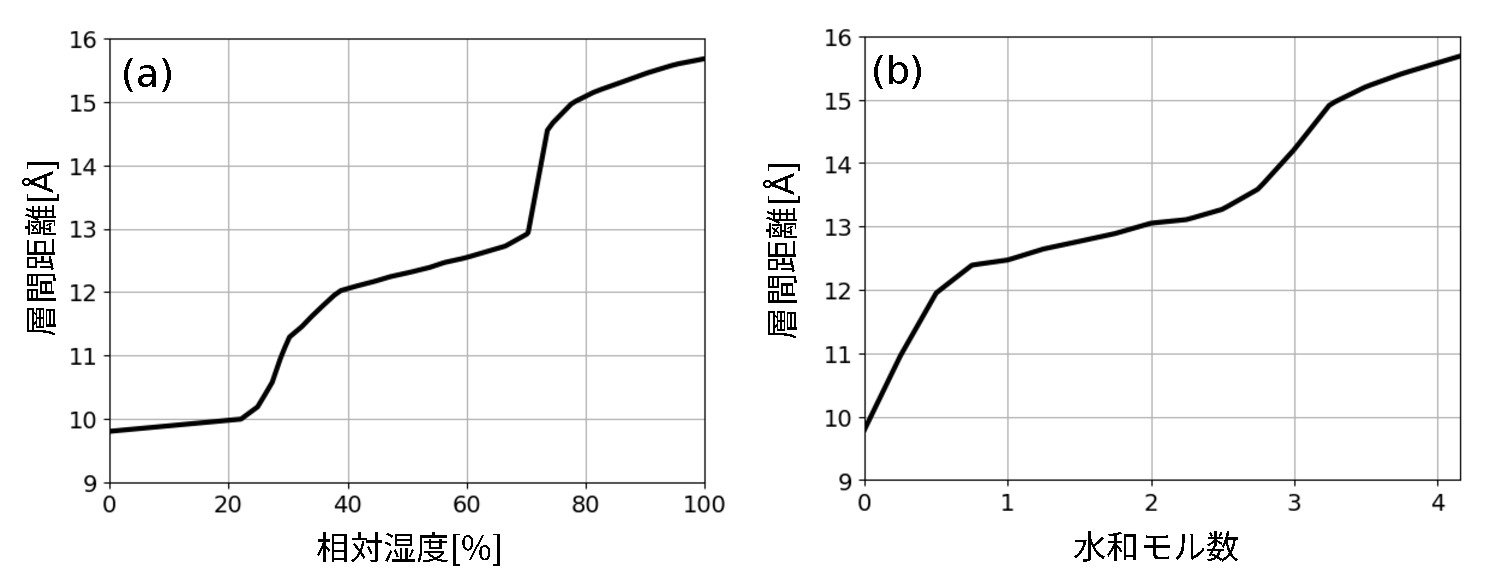
\includegraphics[width=1.0\linewidth]{Figs/fig1.eps} 
	\end{center}
	\caption{
		単調減少する水和エネルギーのモデル(単調モデル).
		$u_{\infty}$は$s\rightarrow \infty$での大きさ.$s_b$は$u=\frac{1}{2}u_{\infty}$となる
		水和層厚さを表す.
	} 
	\label{fig:fig1}
\end{figure}
%--------------------
\begin{figure}[h]
	\begin{center}
%	\includegraphics[width=1.0\linewidth]{Figs/fig2.eps} 
	\end{center}
	\caption{
		水和エネルギーモデルとその成分(内訳).
		(a)振動モデル(i)と単調モデル(ii).
		(b)振動モデル(ii)の成分:単調(青)および振動成分(緑).
		赤は平滑化して振動成分を与えるために用いた三角波.
	} 
	\label{fig:fig2}
\end{figure}
%--------------------
